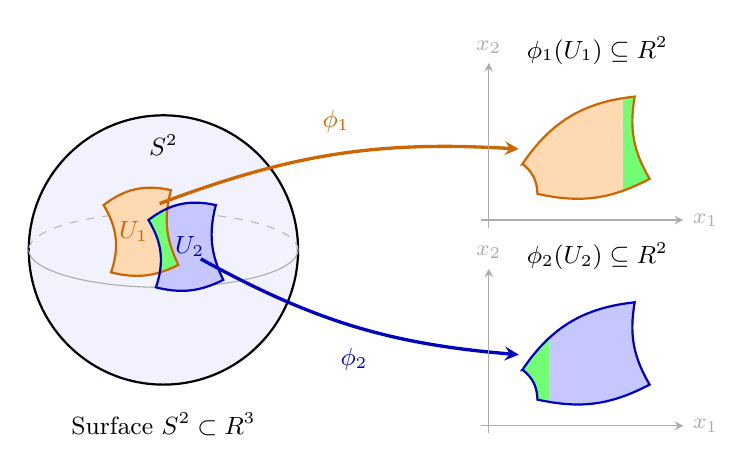
\begin{tikzpicture}[>=stealth, scale=0.95]
  % Reuse each boundary for its fill, overlap clipping, and outline.
  \def\surfacepatchone{(-0.8,0.6) to[bend left=25] (0.1,0.8)
    to[bend right=20] (0.2,-0.2) to[bend left=20] (-0.7,-0.3)
    to[bend right=25] cycle}
  \def\surfacepatchtwo{(-0.2,0.4) to[bend left=25] (0.7,0.6)
    to[bend right=20] (0.8,-0.4) to[bend left=20] (-0.1,-0.5)
    to[bend right=25] cycle}
  \def\flatpatch{(-0.8,-0.2) to[bend left=25] (0.7,0.7)
    to[bend right=20] (0.9,-0.4) to[bend left=20] (-0.6,-0.6)
    to[bend right=25] cycle}

  % Nearby irregular surface patches with a small shared region.
  \draw[thick, fill=blue!5] (0,0) circle (1.8);
  \draw[dashed, gray!55] (1.8,0) arc (0:180:1.8 and 0.5);
  \draw[gray!65] (-1.8,0) arc (180:360:1.8 and 0.5);
  \node[font=\small] at (0,1.4) {$S^2$};

  \fill[orange!30] \surfacepatchone;
  \fill[blue!22] \surfacepatchtwo;
  \begin{scope}
    \clip \surfacepatchone;
    \clip \surfacepatchtwo;
    \fill[green!55] (-1.0,-0.6) rectangle (1.2,1.0);
  \end{scope}
  \draw[thick, orange!80!black] \surfacepatchone;
  \draw[thick, blue!75!black] \surfacepatchtwo;
  \node[font=\small, text=orange!80!black] at (-0.4,0.25) {$U_1$};
  \node[font=\small, text=blue!75!black] at (0.35,0.05) {$U_2$};
  \node[below, font=\small] at (0,-2.05) {Surface $S^2\subset\mathbb{R}^3$};

  % Each patch has its own flat map, shown with two coordinate axes.
  \draw[->, very thick, orange!80!black]
    (-0.05,0.62) to[bend left=12]
    node[above=4pt, font=\small] {$\phi_1$} (4.75,1.35);
  \draw[->, very thick, blue!75!black]
    (0.5,-0.12) to[bend right=12]
    node[below=4pt, font=\small] {$\phi_2$} (4.75,-1.4);

  \begin{scope}[shift={(5.6,1.35)}]
    \draw[->, gray!65, thin] (-1.35,-0.95) -- (1.35,-0.95)
      node[right, font=\footnotesize] {$x_1$};
    \draw[->, gray!65, thin] (-1.25,-1.05) -- (-1.25,1.15)
      node[above, font=\footnotesize] {$x_2$};
    \fill[orange!30] \flatpatch;
    \begin{scope}
      \clip \flatpatch;
      \fill[green!55] (0.55,-0.8) rectangle (1.05,0.9);
    \end{scope}
    \draw[thick, orange!80!black] \flatpatch;
    \node[font=\small, above] at (0.2,1.0)
      {$\phi_1(U_1)\subseteq\mathbb{R}^2$};
  \end{scope}

  \begin{scope}[shift={(5.6,-1.4)}]
    \draw[->, gray!65, thin] (-1.35,-0.95) -- (1.35,-0.95)
      node[right, font=\footnotesize] {$x_1$};
    \draw[->, gray!65, thin] (-1.25,-1.05) -- (-1.25,1.15)
      node[above, font=\footnotesize] {$x_2$};
    \fill[blue!22] \flatpatch;
    \begin{scope}
      \clip \flatpatch;
      \fill[green!55] (-1.05,-0.8) rectangle (-0.45,0.9);
    \end{scope}
    \draw[thick, blue!75!black] \flatpatch;
    \node[font=\small, above] at (0.2,1.0)
      {$\phi_2(U_2)\subseteq\mathbb{R}^2$};
  \end{scope}
\end{tikzpicture}
